\chapter{รายละเอียดการปฏิบัติงาน}
\label{chapter:related-theory}

\section{ตำแหน่งและลักษณะงานที่นักศึกษาได้รับมอบหมาย}

ตำแหน่ง: Full Stack Developer

\subsection{งานที่ได้รับผิดชอบ}

\begin{enumerate}
  \item ศึกษาเทคโนโลยีที่มีคุณภาพเพื่อประยุกต์ใช้กับการทำงาน
  \item พัฒนาเว็บแอพพลิเคชั่นประเมินความสามารถเบื้องต้นของผู้สมัครงาน
  \item ควบคุมคุณภาพของโค้ดให้มีคุณภาพที่ดี
\end{enumerate}

\section{รายละเอียดของโครงการที่ได้รับผิดชอบ}

เนื่องจากนักศึกษาได้รับหน้าที่ในตำแหน่ง Developer ในทีม BUDDY RECRUIT ซิ่งทำเกี่ยวกับการช่วยให้บริษัทหาคนเข้ามาทำงาน ได้ตรงตามความต้องการของบริษัท จึงได้รับมอบหมายให้ทำเว็บแอพพลิเคชั่นประเมินความสามารถเบื้องต้นของผู้สมัครงาน โดยเว็บแอพพลิเคชั่นนี้ช่วยให้คัดกรองผู้คนได้มีประสิทธิภาพมากยื่งขึ้น ผ่านการทำข้อสอบที่สามารถกำหนดระดับความยากของข้อสอบได้ และดึงคลังคำถามมาแบบสุ่ม ส่งให้ผู้ทำข้อสอบโดยอัติโนมัติผ่านทางอีเมล เมื่อผู้สมัครงานทำข้อสอบเสร็จแล้ว ข้อสอบจะถูกส่งไปที่ผู้ออกข้อสอบ พร้อมตรวจข้อที่เป็นคำถามปรนัยให้อัตโนมัติ โดยระบบนี้แบ่งเป็น 2 ส่วนหลักๆ ได้แก่

\begin{enumerate}
  \item ส่วนต่อประสานกับผู้ใช้(Front-end) เป็นส่วนที่ผู้ใช้งานสามารถมีปฏิสัมพันธ์กับเว็บแอพพลิเคชั่นได้ ผ่าน UI(User Interface) ที่หน้าเว็บแอปพลิเคชั่น
  \item ส่วนที่จัดการกับฐานข้อมูล(Back-end) เป็นส่วนที่ผู้ใช้งานไม่สามารถมองเห็นได้จากภายนอก เป็นการทำงานหลักๆของเว็บแอพพลิเคชั่น เช่น การเก็บข้อมูล การเรียกใช้ข้อมูล และการเชื่อมต่อการทำงานร่วมกับระบบอื่นๆ
\end{enumerate}

อนึ่ง ข้อมูลข้างต้นเป็นเพียงภาพรวมของเว็บแอพพลิเคชั่นโดยย่อ ซึ่งรายละเอียดของเว็บแอพพลิเคชั่นนี้จะกล่าวโดยละเอียดในบทถัดไป

\section{แนวคิดและทฤษฏีที่เกี่ยวข้อง}

\subsection{RESTful Web Services (RWS)}

เป็น web service ที่ใช้ REST architectural style โดยจะอนุญาติให้ระบบ Request และเข้าถึง Resource บนเว็บโดยใช้ชุดคำสั่งที่กำหนดเอาไว้  การตอบโต้ของ REST อยู่บนพื้นฐานของ Hypertext Transfer Protocol (HTTP) โดย Request จะส่งคำขอไปยัง URI ที่กำหนด และส่งข้อมูลกลับมาในรูปแบบ HTML, XML, JSON หรือ format อื่นๆ ทำให้สามารถบำรุงรักษาง่าย และสามารถ scale service ได้~\cite{Guru99}

\begin{itemize}
  \item Client-server architecture: Client ผู้ที่เข้ามาขอ resources ไม่ต้องรู้ Business logic ภายใน ส่วน Server มีหน้าที่เก็บข้อมูล ไม่จำเป็นต้องรู้เกี่ยวกับ UI หรือสถานะของผู้เรียก
  \item Stateless: ส่ง request ให้เซิร์ฟเวอร์แล้วรับกลับมาเป็น response เมื่อรับ response มาแล้วจบการทำงาน
  \item Cache: สามารถกำหนดได้ว่าจะเก็บ cache ของ response นั้นหรือไม่
  \item Layered system: สามารถปรับปรุงความสามารถในการขยายระบบได้ โดยการใช้งานการทำ Load balance
  \item Interface/Uniform Contract: วิธีการที่จะคุยกับเซิร์ฟเวอร์โดยไม่คำนึงถึงประเภทของอุปกรณ์ หรือประเภทของแอพพลิเคชั่น
\end{itemize}

\subsection{HTTP Request}

HTTP คือ protocol ที่อนุญาติให้ไคลเอนต์ดึงข้อมูลจากเซิร์ฟเวอร์~\cite{Guru99}

\begin{itemize}
  \item Request-Line คือส่วนที่ระบุ HTTP Method, Request-URI และ version ของ protocol เช่น HTTP/1.0, HTTP/1.1, HTTP/2.0
  \item Headers คือส่วนที่อนุญาติให้ใส่ข้อมูลเพิ่มเติม หรือกฏเกณฑ์ต่างๆเกี่ยวกับการ request เช่น รูปแบบของข้อมูล, การเข้ารหัส
  \item Body คือส่วนที่ระบุข้อมูลที่ต้องการจะส่งให้ปลายทาง สามารถส่ง patameter ต่างๆ ไปใน Body เพื่อเพิ่ม, ลบ หรือแก้ไขข้อมูลบนเซิร์ฟเวอร์ได้
\end{itemize}

\subsection{HTTP Request Methods}

คือส่วนที่ใช้ในการกำหนดประเภทของคำร้องขอต่างๆ บน HTTP Request~\cite{Guru99} โดยมี 4 Methods หลักคือ 

\begin{itemize}
  \item POST สำหรับใช้เพื่อสร้างค่าใหม่ เช่น สร้างรายชื่อพนักงานใหม่
  \item GET สำหรับขอข้อมูลจากเซิร์ฟเวอร์ เช่น ขอข้อมูลพนักงานทั้งหมด
  \item PUT สำหรับแก้ไขค่าต่างๆบนเซิร์ฟเวอร์ โดยส่งมาใน body ของ HTTP Request เช่น แก้ไขข้อมูลของพนักงาน
  \item DELETE สำหรับลบค่าบนเซิร์ฟเวอร์ เช่น ลบข้อมูลของพนักงาน
\end{itemize}

\subsection{HTTP Response Status Code}

คือมาตรฐานสถานะที่เซิร์ฟเวอร์ตอบสนองกับเว็บไซต์ต่างๆ~\cite{httpResponse}

\begin{itemize}
  \item 2xx (Successful) 
  
  Request ที่ไคลเอนต์ส่งไปยังเซิร์ฟเวอร์ถูกประมวลผลเรียบร้อย และไม่มี error ใดๆ ประกอบด้วย

  200 : (OK) ส่ง request สำเร็จ

  201 : (Created) ผู้ใช้สร้างข้อมูลลง database สำเร็จ response นี่จะได้รับหลัง POST หรือ PUT requests

  202 : (Accepted) request สำเร็จแล้วแต่ เซิร์ฟเวอร์ยังประมวลผลไม่เสร็จ
  
  203 : (Non-Authoritative Information) เซิร์ฟเวอร์ประมวลผลสำเร็จแล้ว แต่ทำการส่งข้อมูลมาจากแหล่งอื่น

  204 : (No Content) เซิร์ฟเวอร์ประมวลสำเร็จแล้ว แต่ไม่มีข้อมูลที่ต้องส่งคืนไป

  206 : (Partial Content) เซิร์ฟเวอร์ส่งข้อมูลบางส่วน ตามที่คลเอนต์ต้องการ โดยกำหนดขอบเขตที่ต้องการผ่าน headers บน HTTP Request

  \item 3xx (Redirection)
  
  request ที่ไคลเอนต์ส่งไปหาเซิร์ฟเวอร์ แล้วถูก redirect ส่งไปประมวลผลที่อื่น เพื่อทำให้กระบวน \\ การทำงานสำเร็จ

  300 : (Multiple Choices) request ที่ไคลเอนต์ส่งไปมี response มากกว่า 1 ตัว ไคลเอนต์สามารถเลือกลิงค์ที่จะ redirect ไปได้

  301 : (Moved Permanently) URL ที่ทำการ request ขอข้อมูลถูกดปลี่ยนไปถาวร จึง response ออกมาเป็น URL ใหม่

  302 : (Found) URL ที่ทำการ request มีการเปลี่ยนชั่วคราว

  303 : (See Other) request ที่เรียกอยู่ภายใต้ URL อื่น

  304 : (Not Modified) response นี้ยังไม่ถูกแก้ไข ดังนั้น ไคลเอนต์จะได้รับ response ที่เป็น cached version

  \item 4XX (Client Error)
  
  เกิด error มาจาก request ของไคลเอนต์ที่ผิดพลาด เช่น ผิด URL หรือผิด syntax

  400 : (Bad Request) ไคลเอนต์เขียน syntax ผิด หรือ ไม่ถูกรูปแบบ ทำให้เซิร์ฟเวอร์ไม่เข้าใจ

  401 : (Unauthorized) ไคลเอนต์ต้องทำการยืนยันตัวตนก่อนที่จะได้รับ response

  403 : (Forbidden) ไคลเอนต์ทำการยืนยังตัวตนแล้ว แต่ไม่มีสิทธิ์ในการเข้าถึงข้อมูลนี้

  404 : (Not Found) ถ้าเกิดบน browser คือ URL ไม่ถูกจดจำบนเซิร์ฟเวอร์ แต่ถ้าเกิดบน API  คือ มีการขอข้อมูลที่ถูกต้อง แต่ไม่มีข้อมูลนี้อยู่

  405 : (Method Not Allowed) method ที่เรียกใช้ไม่ถูกต้อง

  406 : (Not Acceptable) header ที่ไคลเอนต์ request ไม่สัมพันธ์กับเซิร์ฟเวอร์

  413 : (Payload Too Large) request ที่ขอใหญ่กว่า limit ที่เซิร์ฟเวอร์กำหนดไว้

  414 : (URI Too Long) URL ที่ทำการ request โดยไคลเอนต์ ยาวกว่าที่เซิร์ฟเวอร์จะยอมรับได้

  415 : (Unsupported Media Type) เซิร์ฟเวอร์ไม่รองรับ media (รูป หรือ สื่อต่างๆ) ดังนั้นเซิร์ฟเวอร์จึงปฏิเสธการ request

  \item  5XX (Server Error)
  
  เซิร์ฟเวอร์มีปัญหา

  500 : (Internal Server Error) เซิร์ฟเวอร์เจอกับสถานการณ์ที่ไม่สามารถจัดการได้

  501 : (Not Implemented) ไคลเอนต์เรียก request method ที่เซิร์ฟเวอร์ไม่รองรับ และเซิร์ฟเวอร์ไม่สามารถจัดการได้

  502 : (Bad Gateway) เซิร์ฟเวอร์เป็น gateway หรือ proxy ได้รับ response ที่ผิดพลาดจากเซิร์ฟเวอร์อื่น

  503 : (Service Unavailable) เซิร์ฟเวอร์อยู่ระหว่างการปรับปรุง หรือยังไม่พร้อมที่จะจัดการ request

  504 : (Gateway Timeout) เซิร์ฟเวอร์เป็น gateway และไม่สามารถ response ข้อมูลในเวลาที่กำหนดได้

\end{itemize}

\subsection{MVC (Model View Controller)}

คือ software design pattern ที่แยกการทำงานขอโปรแกรมออกเป็น 3 ส่วนเพื่อแยกข้อมูลภายในโปรแกรมกับข้อมูลที่แสดงให้ผู้ใช้เห็น~\cite{mvc}

\begin{itemize}
  \item Model คือส่วนที่เป็นโครงสร้างของข้อมูล กำหนดกฎเกณฑ์ของการเก็บข้อมูล และเป็นส่วนที่ไว้สำหรับการจัดการข้อมูลโดยตรง
  \item View คือส่วนที่ไว้แสดงผลตามที่ผู้ใช้ต้องการ ผู้ใช้สามารถเปลี่ยนแปลงข้อมูลที่ผู้ใช้เห็นได้
  \item Controller คือส่วนที่ไว้จัดการกับ Model โดยขึ้นอยู่กับการกระทำของ View ที่กำหนดโดยผู้ใช้ และสรรหาข้อมูลจาก Model เพื่อไปแสดงใน View
\end{itemize}

\begin{figure}[H]
  \centering
  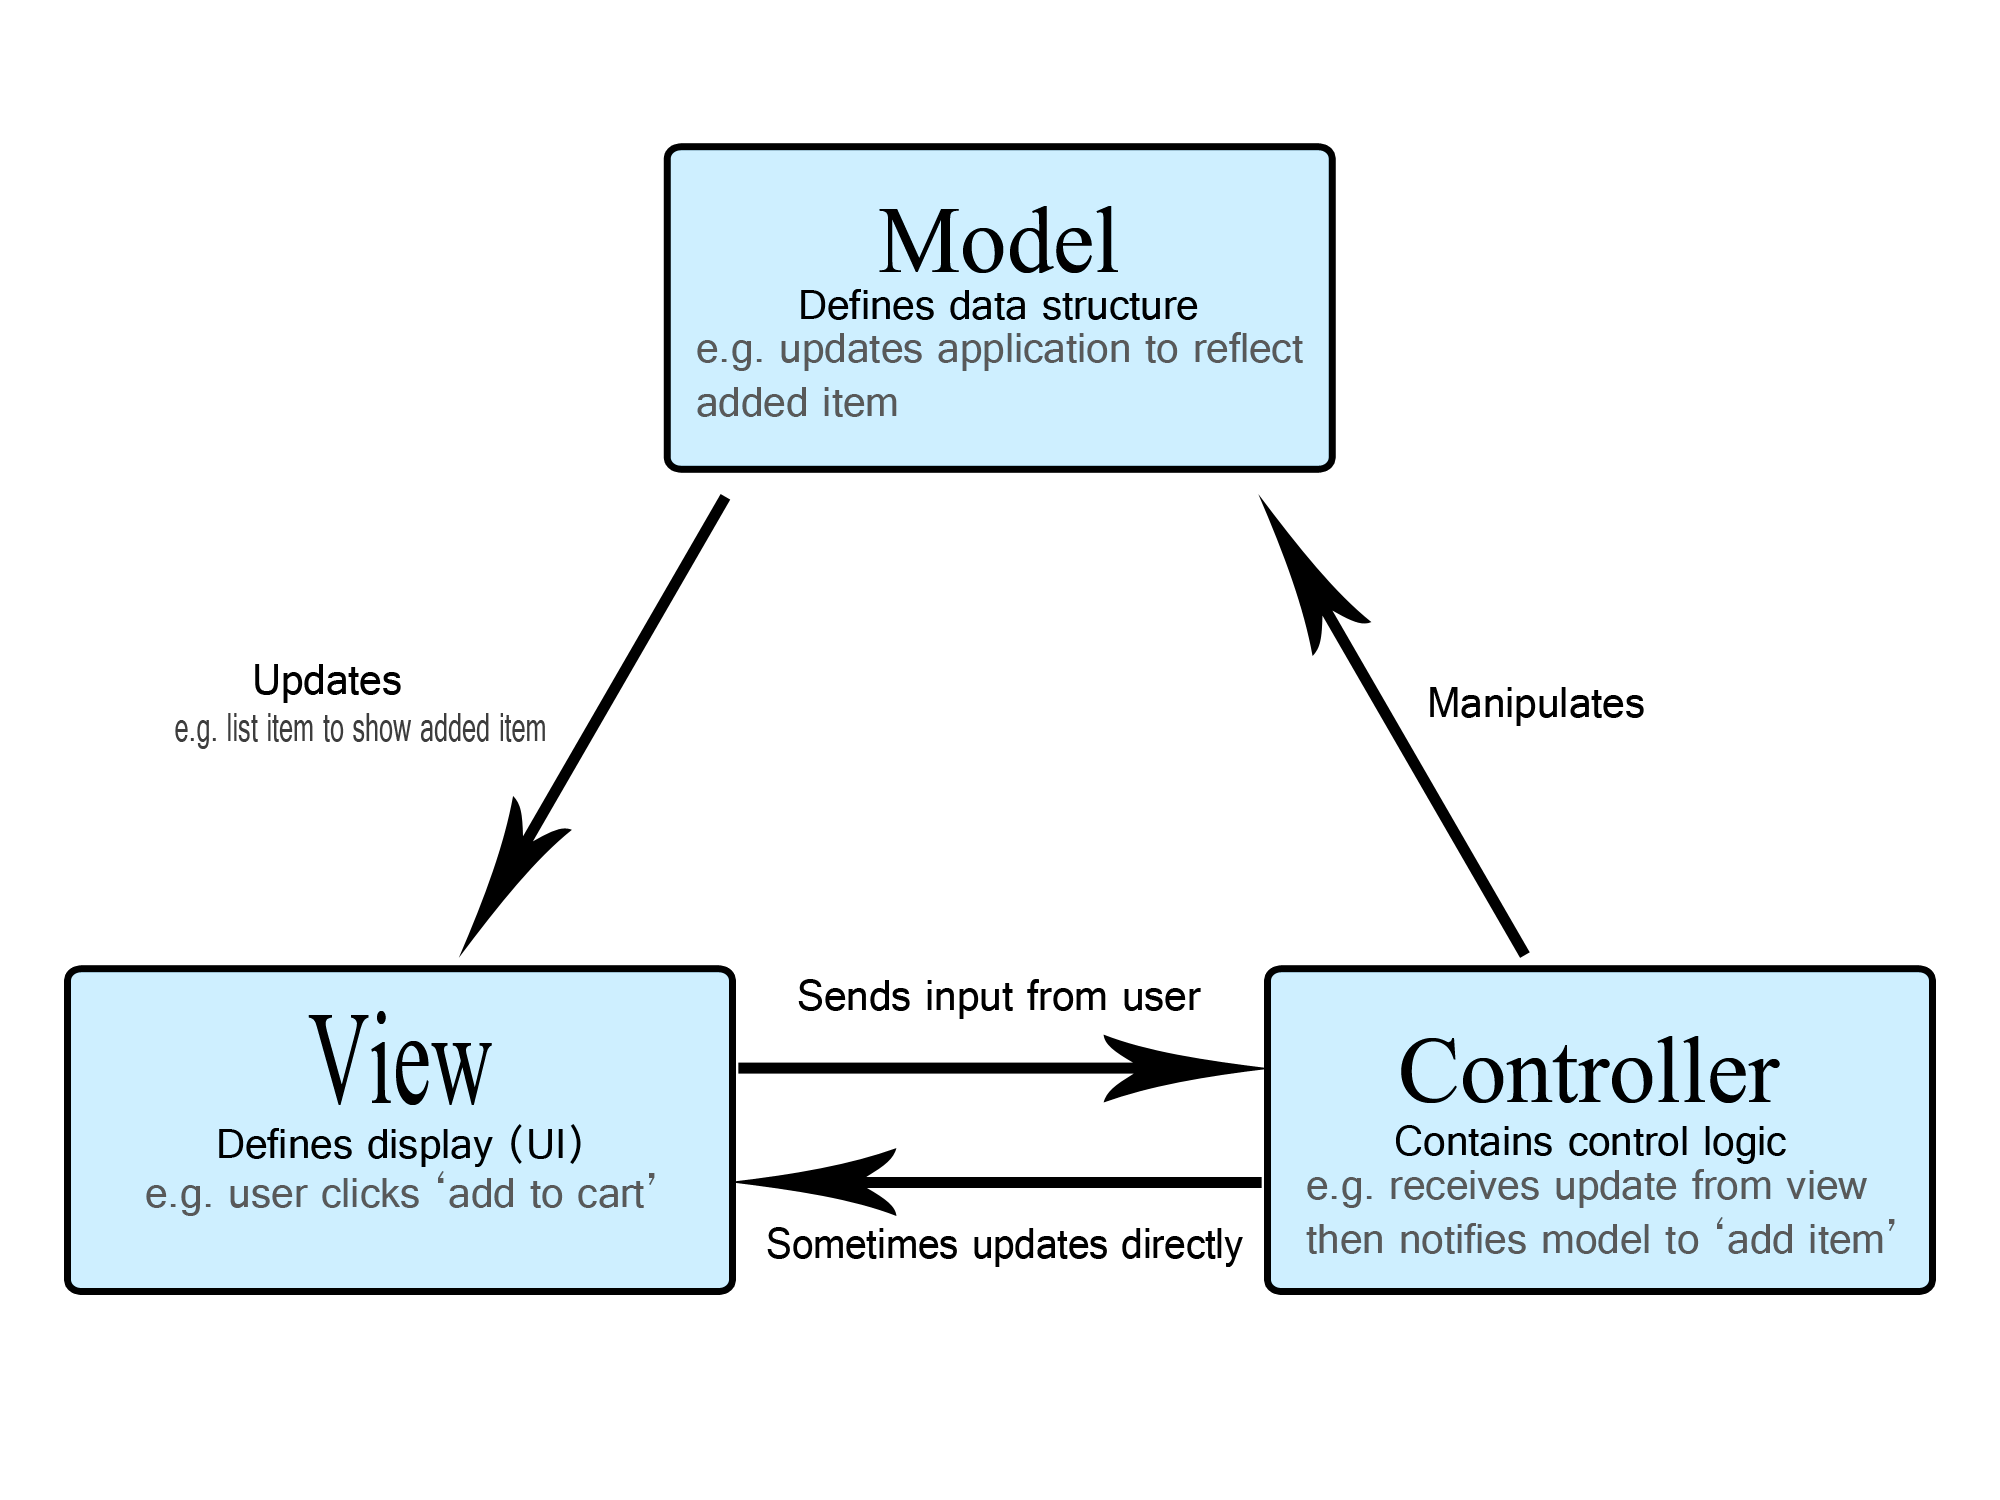
\includegraphics[width=0.8\columnwidth]{model-view-controller.png}
  \caption{แสดง MVC architecture}
  \label{Fig:model-view-controller}
\end{figure}

\subsection{NoSQL Database}

คือ ฐานข้อมูลที่สร้างมาเพื่อให้จัดการข้อมูลที่มีความซับซ้อนได้ง่ายขึ้นเมื่อเทียบกับ SQL databases ที่มีการเก็บข้อมูลในที่รูปแบบแน่นอน (structured data) โดยเพิ่มความสามารถในการจัดเก็บข้อมูลในรูปแบบที่ไม่แน่นอน (unstructured data)  ทำให้สามารถเก็บข้อมูลที่ซับซ้อนได้, เพิ่มความสามารถในการขยายระบบในรูปแบบแนวนอน (Horizontal Scalability) เพื่อรองรับปริมาณข้อมูลในปัจจุบัน~\cite{nosql}
\begin{figure}[H]
  \centering
  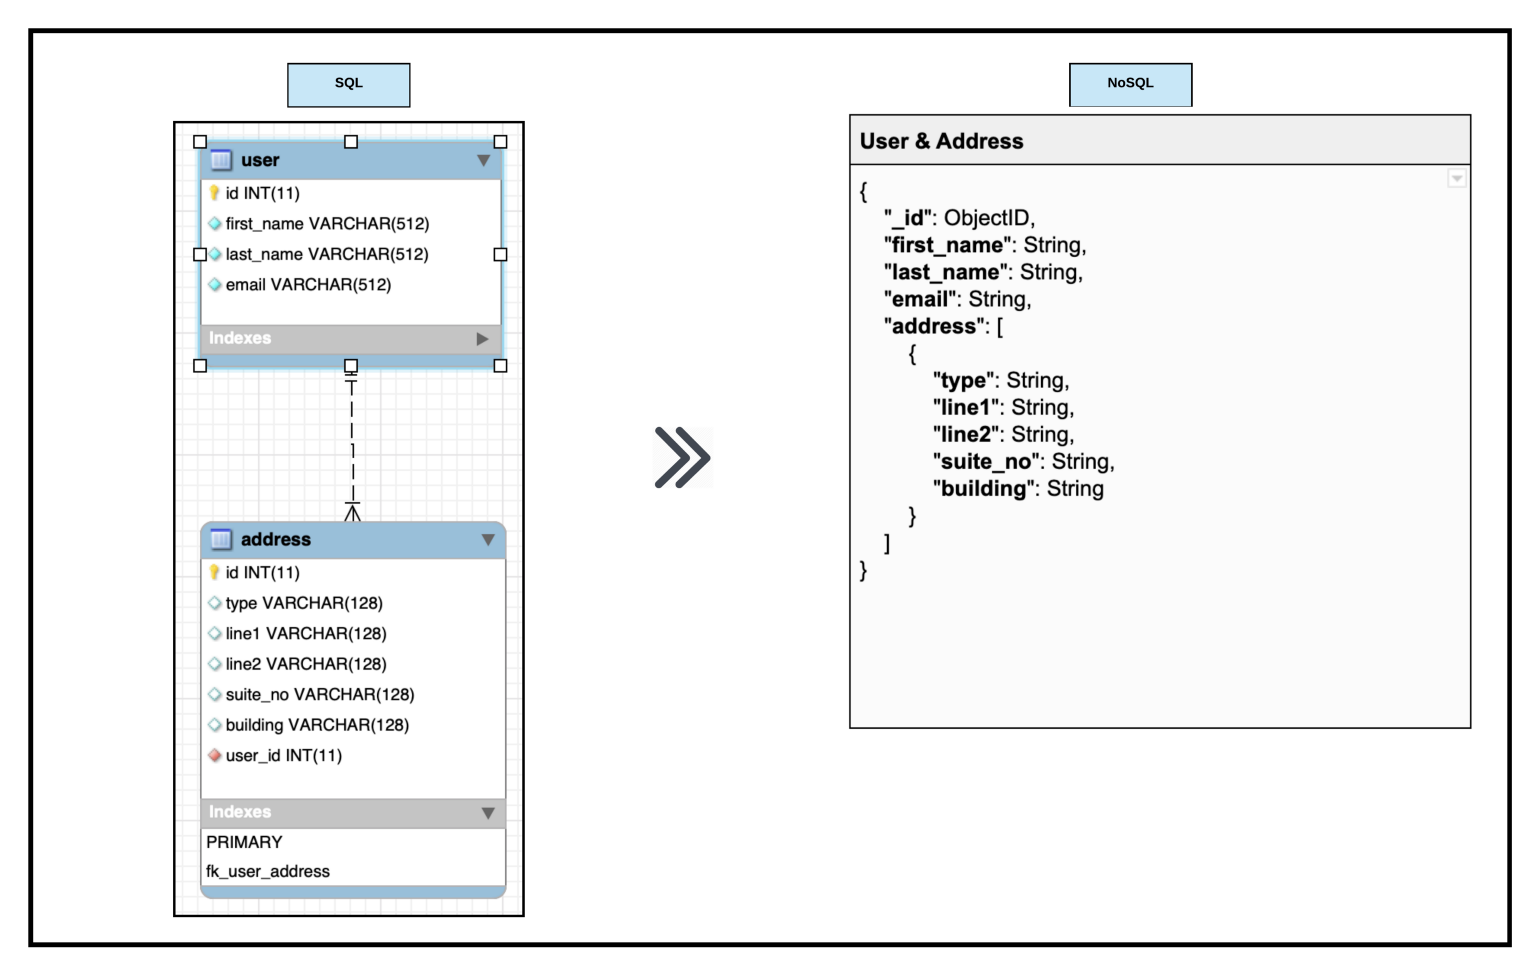
\includegraphics[width=0.9\columnwidth]{no-sql.png}
  \caption{แสดงตาราง SQL เปรียบเทียบกับตาราง NoSQL}
  \label{Fig:no-sql}
\end{figure}

\subsection{Token}

เป็นชุดรหัสเอาไว้ระบุตัวตนของผู้ใช้ว่าผู้ใช้นั้นเป็นใคร ไม่มีรูปแบบที่ตายตัว

\subsection{Container}

เป็นหน่วยของซอฟแวร์ที่ทำการลงทรัพยากรณ์ทุกอย่างที่ต้องใช้ในแอพ และตัวโค้ดของแอพ ดังนั้นแอพพลีเคชั้นจะสามารถถูกเรียกใช้ได้อย่างรวดเร็ว และใช้ในสภาพแวดล้อมใดก็สามารถทำงานได้ โดยมีความเป็นมาตรฐาน และประหยัดทรัพยากรที่ใช้ทำงานตัวแอพพลีเคชั่น~\cite{container}

\subsection{Model–view–viewmodel}

เป็น software architectural pattern รูปแบบที่ช่วยแยกการพัฒนาแอพพลีเคชั่นออกเป็น 3 ส่วน โดยแบ่งออกจากกันอย่างชัดเจนเพื่อให้ง่ายต่อการจัดการและแสดงกระบวนการทำงานในแต่ละส่วน~\cite{mvvm}

\begin{itemize}
  \item Model คือส่วนที่เป็นโครงสร้างของข้อมูล กำหนดกฎเกณฑ์ของการเก็บข้อมูล  และเป็นส่วนที่ไว้สำหรับการจัดการข้อมูลโดยตรง
  \item View คือส่วนที่ไว้แสดงผลตามที่ผู้ใช้ต้องการ ผู้ใช้สามารถเปลี่ยนแปลงข้อมูลได้
  \item View model มีหน้าที่เก็บข้อมูลทั้งหมดที่ View ต้องการ โดย View และ View model มีการใช้ Data-binding ซึ่งกันและกัน กล่าวคือถ้าข้อมูลของ View มีการแก้ไข ข้อมูลของ View model จะได้รับการแก้ไขไปด้วย หรือข้อมูลของ View model มีการแก้ไข ข้อมูลของ View จะได้รับการแก้ไขไปด้วย
\end{itemize}

\begin{figure}[H]
  \centering
  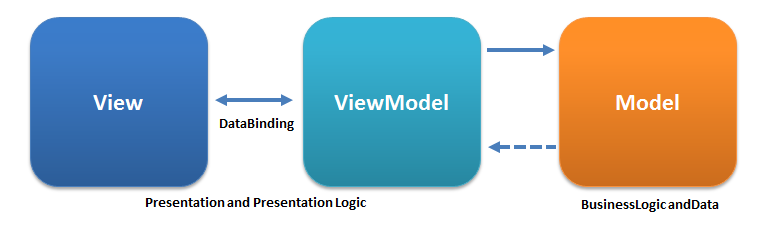
\includegraphics[width=0.9\columnwidth]{MVVMPattern.png}
  \caption{แสดง MVVM architecture}
  \label{Fig:MVVMPattern}
\end{figure}

\newpage

\section{เครื่องมือและเทคโนโลยีที่ใช้ในการปฏิบัติงาน}

\subsection{Trello}

เป็นเว็บแอพพลิเคชั่นที่ช่วยจัดการบริหารโปรเจ็กต์ ให้เป็นระเบียบได้อย่างเรียบง่ายเปรียบเสมือนกระดานไว้วางแผนการทำงาน ระบุรายละเอียดของงานแต่ละงาน โดยเว็บแอพพลิเคชั่นนี้สามารถใช้งานร่วมกันภายในทีมได้ ทำให้การทำงานต่างๆในโปรเจ็กต์มีความคล่องตัวมากยิ่งขึ้น

\begin{figure}[H]
  \centering
  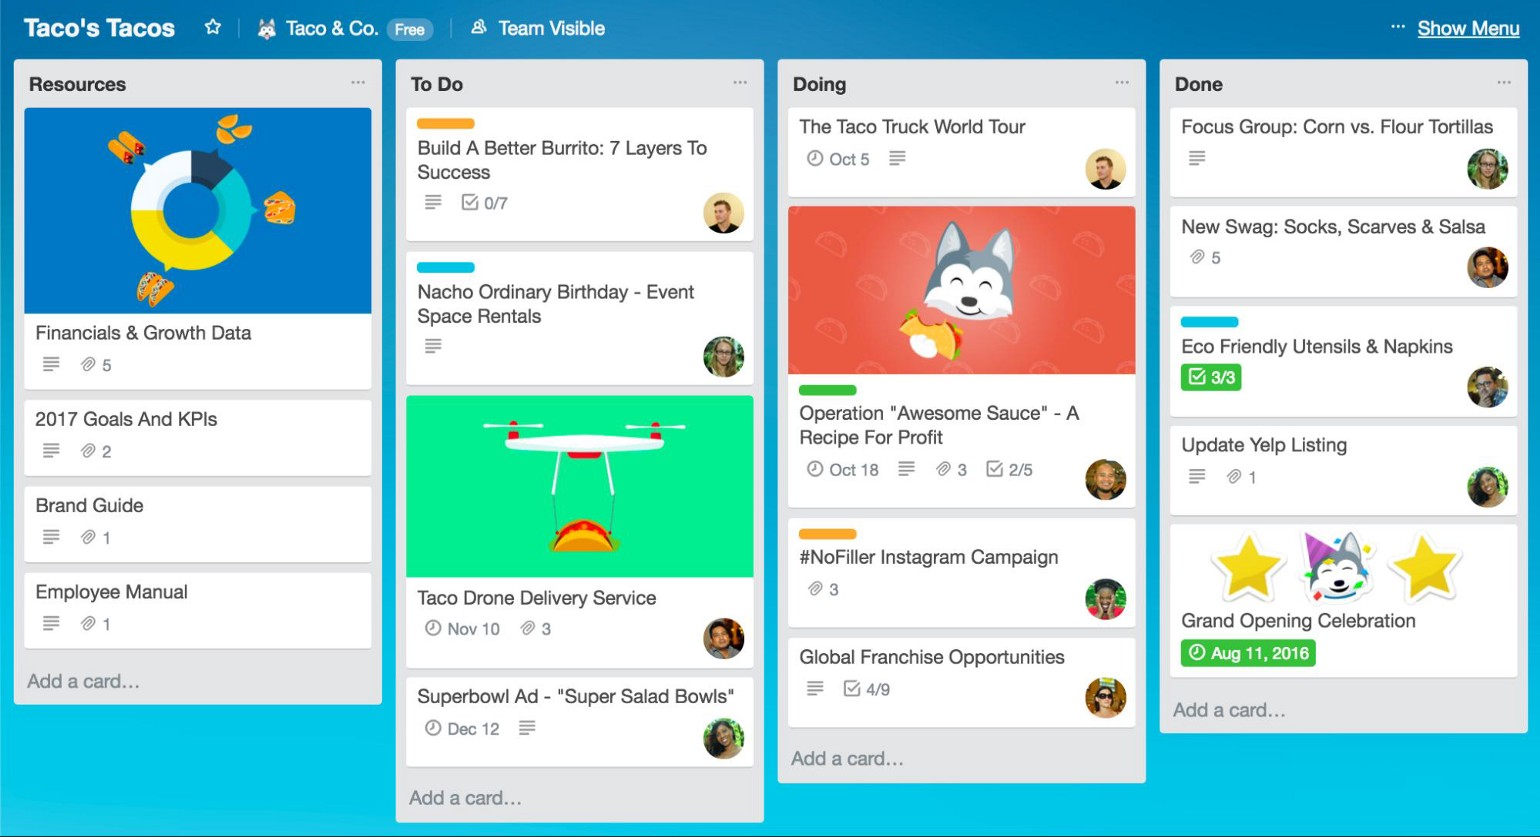
\includegraphics[width=0.9\columnwidth]{trello.png}
  \caption{แสดงตัวอย่างการใช้งาน Trello}
  \label{Fig:trello}
\end{figure}

\subsection{Figma}

เป็นเครื่องมือที่นำมาใช้ในการออกแบบ prototype ของงานที่ทำ โดยสามารถใช้งานแอพพลิเคชั่น Figma ได้ในทุกแพลตฟอร์ม

\begin{figure}[H]
  \centering
  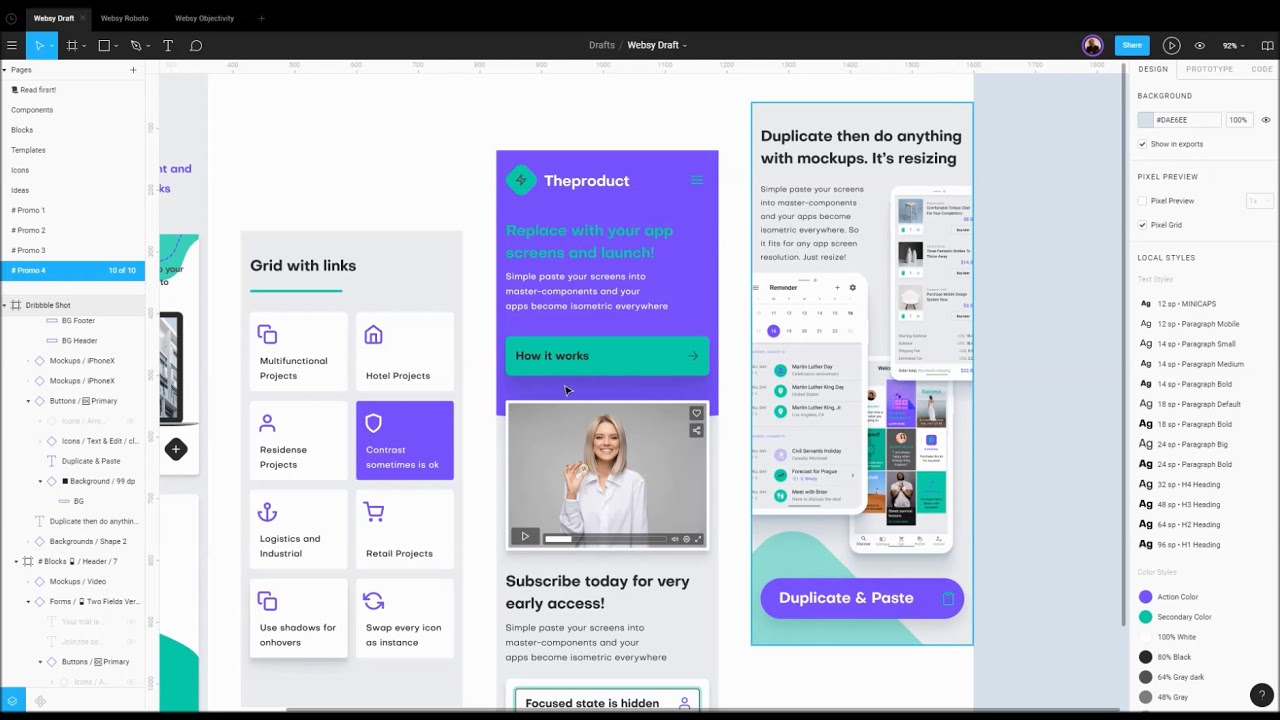
\includegraphics[width=0.9\columnwidth]{figma.jpg}
  \caption{แสดงตัวอย่างการใช้งาน Figma}
  \label{Fig:figma}
\end{figure}

\subsection{Visual Studio Code}

เป็นโปรแกรม code editor ที่ใช้ในการเขียน แก้ไข และปรับแต่งโค้ด โดยพัฒนาออกมาในรูปแบบ OpenSource โดยมีความสามารถในการเปลี่ยนสี Syntax ของโค้ด ตามแต่ละภาษา เพื่อให้ง่ายต้อการมองและการขียนโค้ด ซึ่งสนับสนุนภาษามากมาย ยกตัวอย่างเช่น ภาษา C++, Java, JavaScript, PHP, Python เป็นต้น และยังสามารถติดตั้งส่วนขยายที่เพิ่มความสะดวกสบายในการเขียนโค้ด ตามที่เราต้องการได้

\begin{figure}[H]
  \centering
  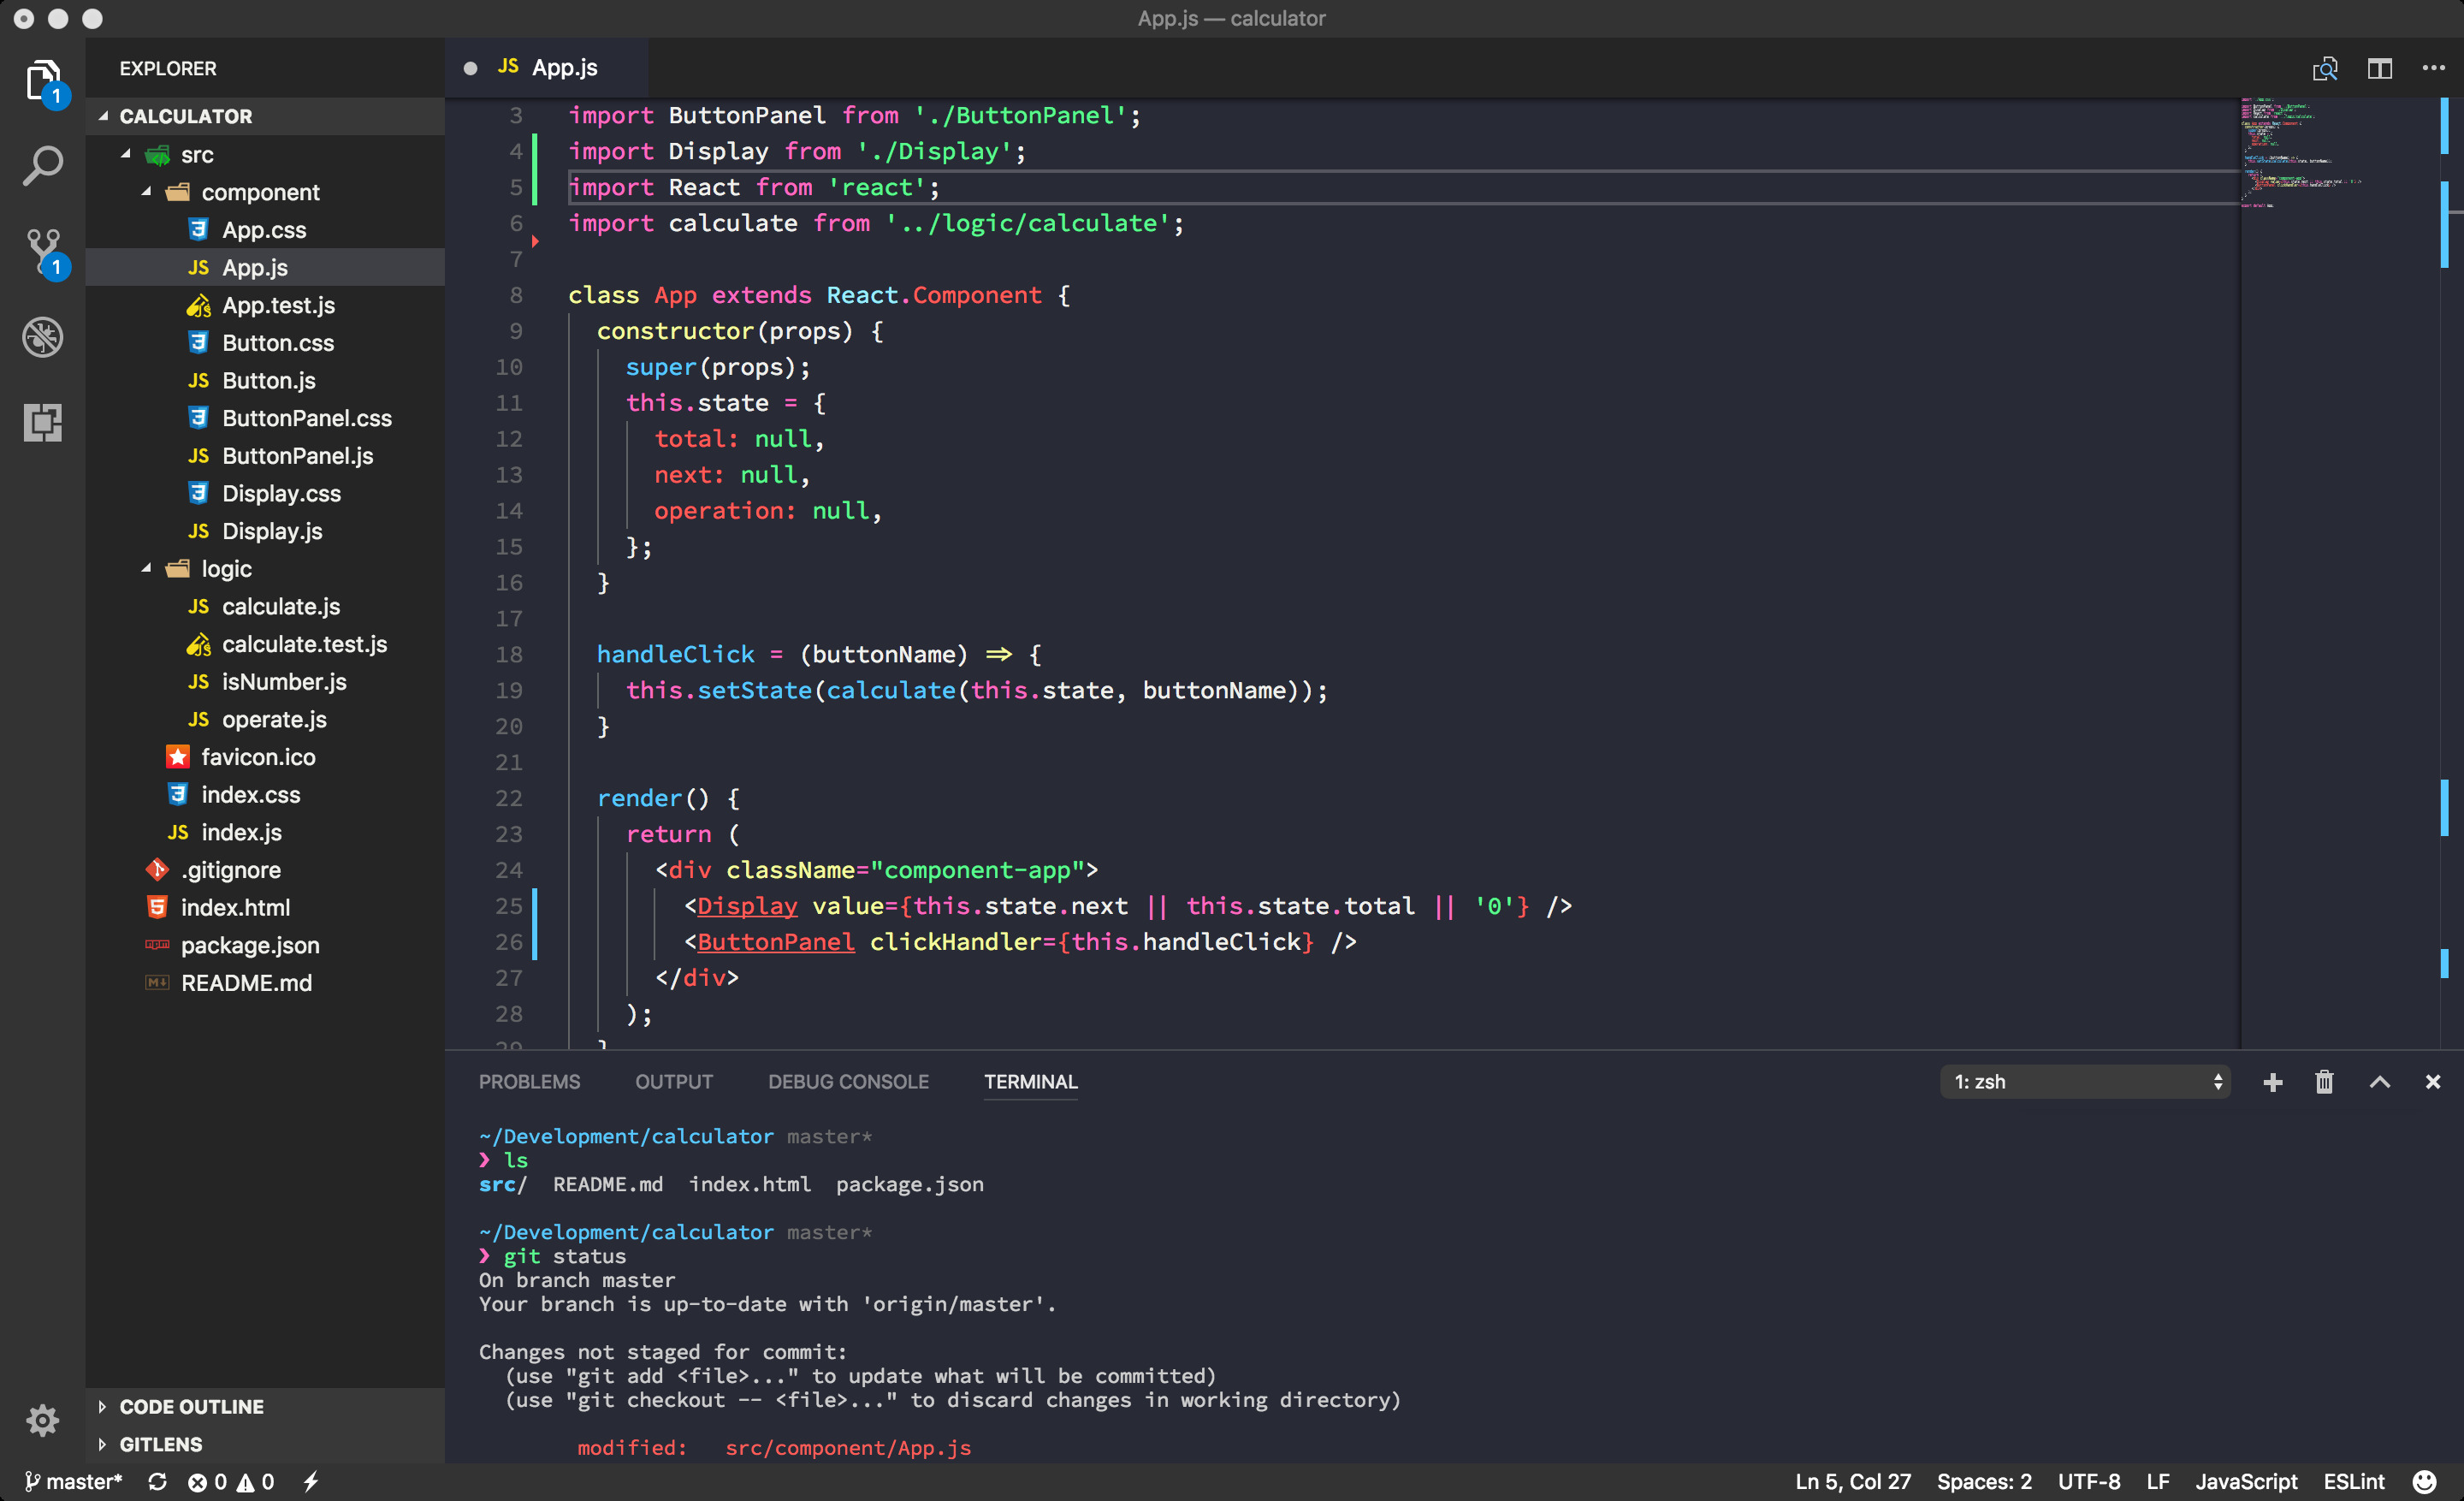
\includegraphics[width=0.9\columnwidth]{vscode.jpg}
  \caption{แสดงตัวอย่างการใช้งาน vscode}
  \label{Fig:vscode}
\end{figure}

\subsection{Vue.js}

เป็น JavaScript Framework ที่สร้างส่วนต่อประสานกับผู้ใช้ (UI) และเป็น single-page applications คือ wep application ที่ทำการโหลด page เพียงครั้งเดียวแต่สามารถเรียกข้อมูลอื่นๆแบบ dynamic ได้ ทำให้ประสบการณ์การใช้งานเว็บใกล้เคียง native app มากยิ่งขึ้น

\subsection{VueX}

เป็น state management pattern ที่ผสมผสานกับ library เพื่อใช้สำหรับจัดการ state เพื่อให้ data flow ของโปรเจคไปในทิศทางเดียวกัน code จึงมีความเป็นระบบมากยิ่งขึ้น และลดการเขียน code ที่ซับซ้อน ทำให้การทำงานร่วมกันภายในทีมสะดวกมากยิ่งขึ้น เช่นการให้คนในทีมรับผิดชอบแต่ละ module~\cite{vuex}

\subsection{Node.js}

เป็น JavaScript runtime กล่าวคือเป็นตัวที่ทำให้ JavaScript  สามารถใช้งานในส่วนของ backend หรือเซิร์ฟเวอร์ได้

\subsection{Express.js}

เป็น Node.js web application framework  ซึ่งมีฟิจเจอร์ต่างๆที่ช่วยให้พัฒนาเซิร์ฟเวอร์ด้วย Node.js ได้สะดวกมากยิ่งขึ้น เช่นการจัดการ request และ response

\subsection{Git}

เป็น Version control ที่เอาไว้ติดตาม และควบการเปลี่ยนแปลงของโค้ดเพื่อให้นักพัฒนา สามารถทำงานร่วมกันได้อย่างมีประสิทธิภาพ~\cite{git}

\subsection{Github}

เป็น website Git (version control repository) สำหรับนักพัฒนาซอฟแวร์ ใช้หลักการทำงานของ git แต่สามารถใช้งานร่วมกับผู้อื่นได้ผ่านอินเตอร์เน็ต

\subsection{Docker}

เป็น engine ที่มีการจำลองสภาพแวดล้อมขึ้นมาบนเครื่องเซิร์ฟเวอร์ เพื่อทำการนำ service ที่ต้องการมาทำงานอยู่บนเซิร์ฟเวอร์ โดยใช้หลักการ container ในการจำลองสภาพแวดล้อมขึ้นมาทำงาน service ของเราโดยที่ไม่ต้องมีการนำ os เข้ามาใช้ ทำให้ service ทำงานในสภาพแวดล้อมใดก็ได้~\cite{container}

\begin{figure}[H]
  \centering
  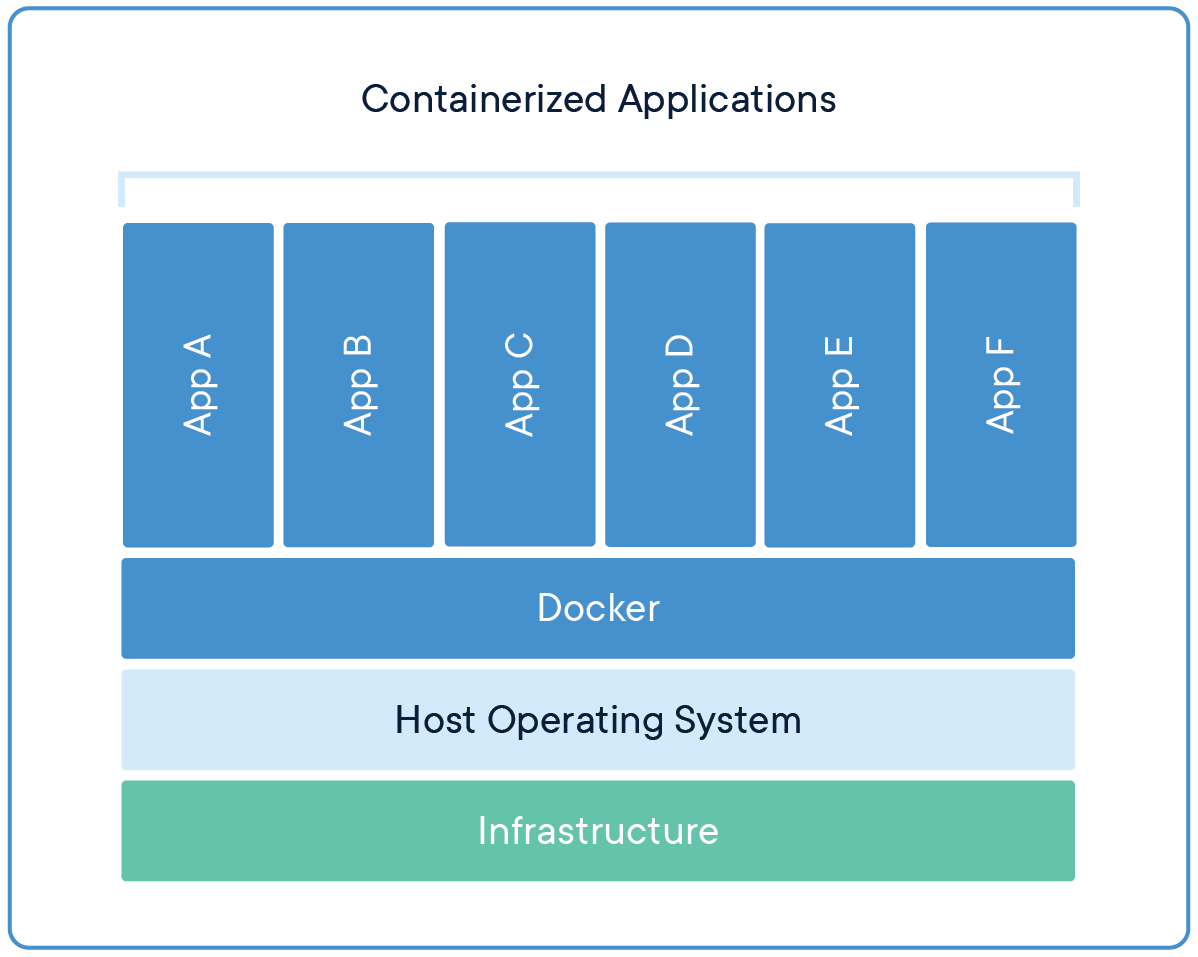
\includegraphics[width=0.8\columnwidth]{docker.png}
  \caption{แสดงตัวอย่างการทำงานของ docker}
  \label{Fig:docker}
\end{figure}

\subsection{Kubernetes}

Kubernetes เป็น Orchestration ที่มาช่วยในการ จัดการคอนเทนเนอร์ ซึ่งหน้าที่หลักๆคือช่วยให้สามารถติดตั้ง(Deployment) จัดสรรทรัพยากรหรือเพิ่มลดทรัพยากรแบบอัตโนมัติได้(Managing \& Scaling) และสามารถใช้งานได้อย่างต่อเนื่องตามที่เราต้องการ ด้วยระบบที่พร้อมใช้งานตลอดเวลา(Auto Self-Healing) โดยในการตั้งค่าต่างๆ ให้กับ Kubernetes สามารถทำได้ด้วยการสร้างไฟล์ .yaml หรือ .yml โดยรูปที่ 2.8 จะเป็นตัวอย่างของไฟล์ .yaml ที่เอาไว้ตั้งค่า Kubernetes \cite{kube}

\begin{figure}[H]
  \centering
  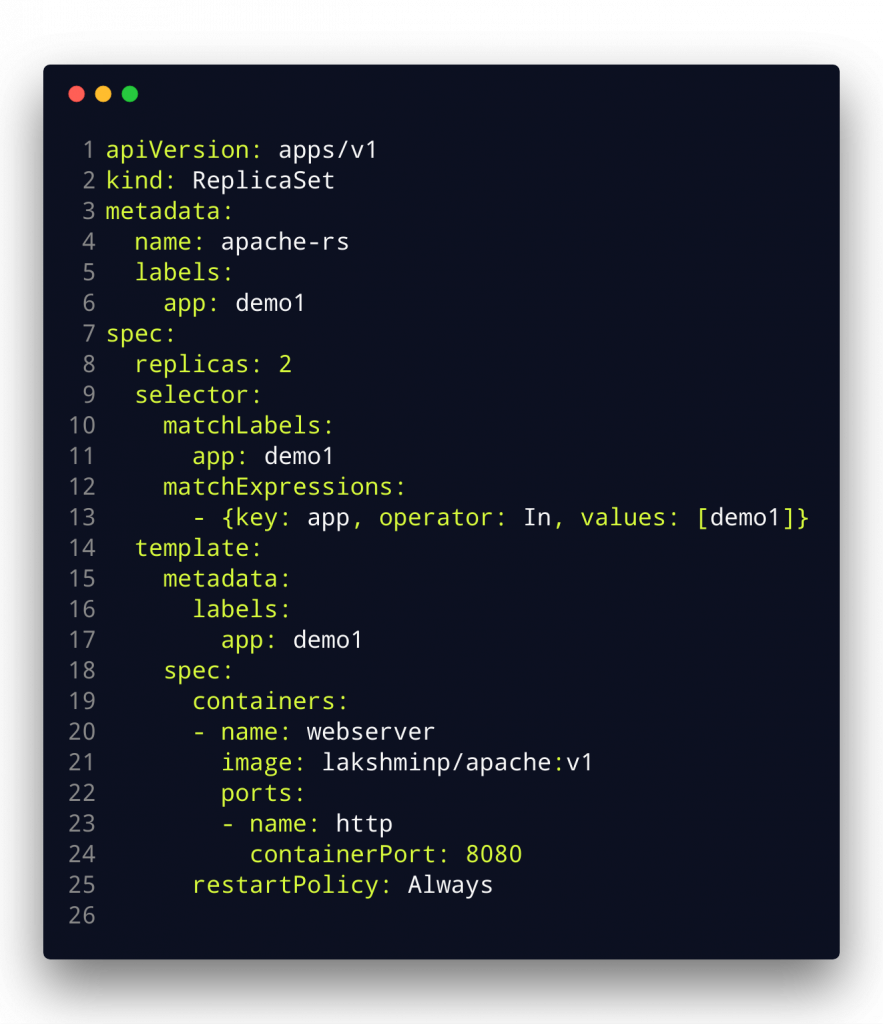
\includegraphics[width=0.9\columnwidth]{kubeExample.png}
  \caption{แสดงตัวอย่างการใช้งาน Kubernetes}
  \label{Fig:kubernetes}
\end{figure}

\subsection{Postman}

เป็นเครื่องมือที่มาช่วยในการ API เพิ่อทดสอบการทำงานของ Service โดยมีหน้าตาส่วนต่อประสานกับผู้ใช้(UI) ที่สวยและใช้งานง่าย

\begin{figure}[H]
  \centering
  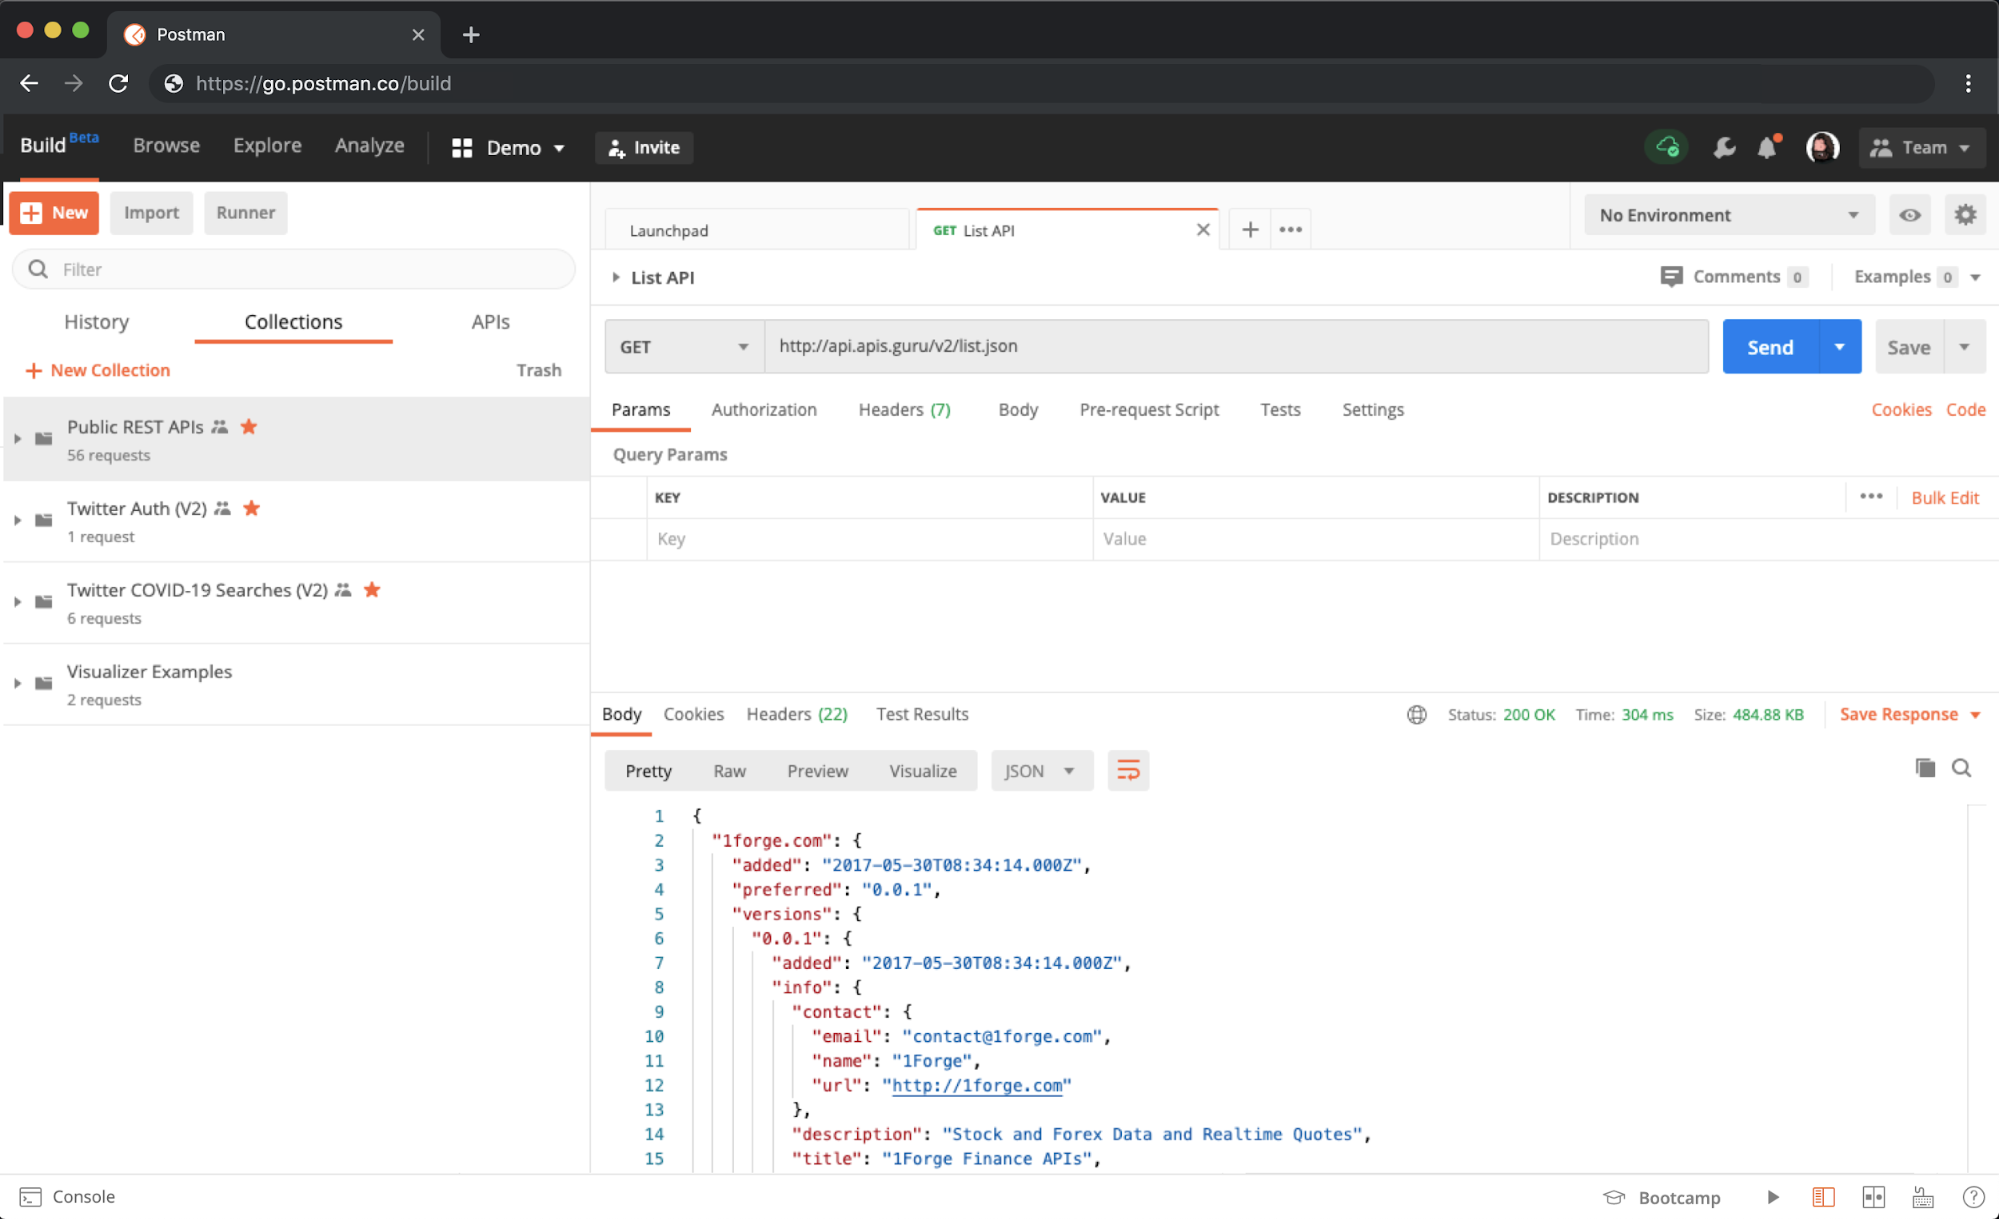
\includegraphics[width=0.9\columnwidth]{postman.png}
  \caption{แสดงตัวอย่างการใช้งาน postman}
  \label{Fig:postman}
\end{figure}

\subsection{JWT (Json Web Token)}

เป็นมาตรฐาน RFC 7519 ในการยืนยันตัวตน (Authentication) ที่เข้ามาแก้ปัญหาการส่งข้อมูลระหว่างกันในวิธีแบบดั้งเดิมคือ Server Based Authentication ที่เปลืองทรัพยากรในการเก็บ Session ID และไม่รองรับการขยายตัว (Scalability)  โดย JWT นั้นสามารถเก็บข้อมูลภายในตัวได้ และมีขนาดที่กระทัดรัด เพื่อนำมาใช้กับ Single Page Web Application (SPA)~\cite{jwt} โดย JWT แบ่งโครงสร้างออกเป็น 3 ส่วน

\begin{enumerate}
  \item Header เก็บประเภทของ token
  \item Payload เก็บข้อมูล
  \item Signature เป็นลายเซ็นที่อยู่ในรูปแบบของอิเล็กทรอนิกส์ (Digital Signed) เพื่อเช็คว่าเป็น token ที่ถูกสร้างอย่างถูกต้องหรือไม่  
\end{enumerate}

\begin{figure}[H]
  \centering
  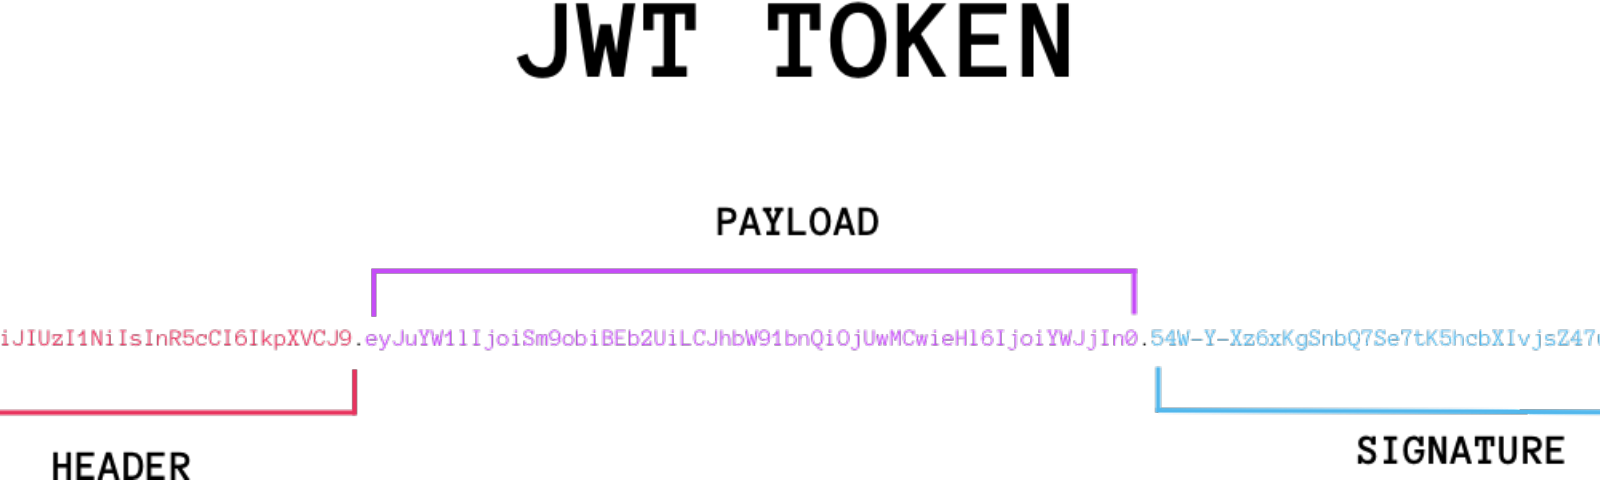
\includegraphics[width=0.9\columnwidth]{jwt.png}
  \caption{แสดงตัวอย่าง jwt endcoded}
  \label{Fig:jwt}
\end{figure}

\subsection{MongoDB}

เป็น open-source document database ประเภทหนึ่ง โดยเก็บข้อมูลแบบ NoSQL Database และเก็บข้อมูลในรูปแบบของ JSON (JavaScript Object Notation) ซึ่งเก็บเป็น key และ value ซึ่งมีสมรรถภาพสูงกว่าการเก็บด้วยโครงสร้างแบบแถวและหลัก(row/column) แบบดั้งเดิม~\cite{mongodb}

\subsection{Robo 3T}

เป็นการใช้ภาพเป็นตัวประสานกับผู้ใช้ของ(GUI) ของ MongoDB ช่วยทำให้ใช้งาน MongoDB ได้สะดวกมากยิ่งขึ้น เช่น เขียน SQL เพื่อ query ข้อมูลใน MongoDB หรือ Import และ export ไฟลล์ข้อมูลเป็น CSV, JSON, SQL and BSON/mongodump ได้~\cite{robo3t}

\begin{figure}[H]
  \centering
  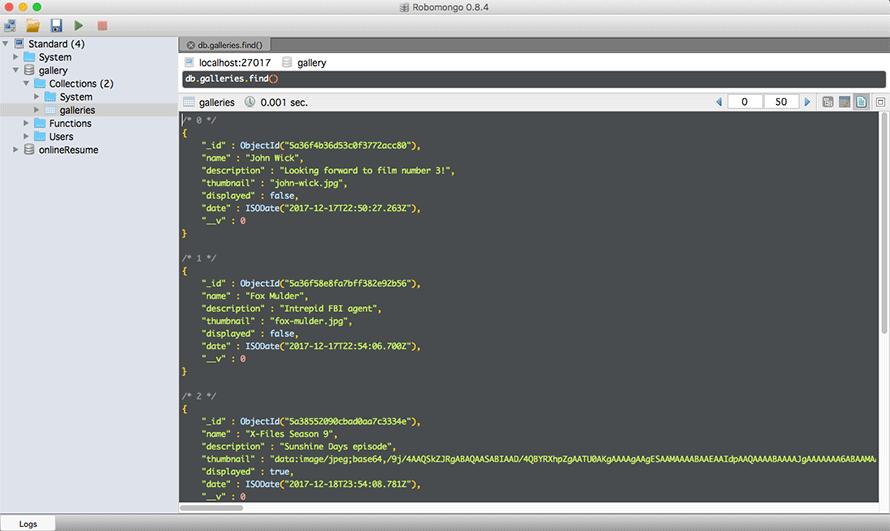
\includegraphics[width=0.9\columnwidth]{robo3t.png}
  \caption{แสดงตัวอย่างการใช้งาน Robo 3T}
  \label{Fig:robo3t}
\end{figure}

\subsection{SendGrid}

เป็น API ช่วยในการส่งอีเมลให้ผู้อื่น สามารถตรวจสอบอีเมลที่ส่งว่าส่งไปถึงหรือไม่ มีปัญหาอะไรเกินขึ้นหรือเปล่า และมีการเก็บสถิติข้อมูลอีเมลท่ีส่ง สรุปออกมาแสดงให้วิเคราะห์เช่น มีการเปิดเมลอ่านกี่ครั้ง มีการรายงานว่าเป็นสแปมกี่ครั้ง

\begin{figure}[H]
  \centering
  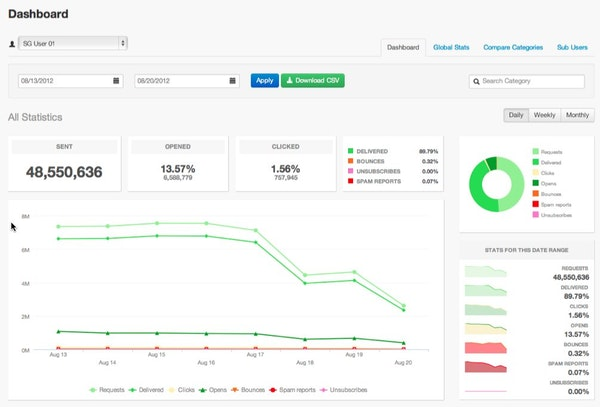
\includegraphics[width=0.9\columnwidth]{sendgrid.jpg}
  \caption{แสดงตัวอย่างสถิติของอีเมลที่ทำการส่งด้วย sendgrid}
  \label{Fig:robo3t}
\end{figure}

\section{ลักษณะขั้นตอนการทํางาน}

--

